\documentclass{amsart} 
\usepackage{graphicx}
\graphicspath{{./}}
\usepackage[fontsize=14pt]{scrextend}
\usepackage{hyperref}
\usepackage{csvsimple}
\usepackage{epigraph}
\title{Zulf's Corporate Dilemma And Inflexibility of Human Nature}
\author{Zulfikar Moinuddin Ahmed}
\date{\today}
\begin{document}
\maketitle

\section{The Importance of Invariance of Attitude Towards Corporations}

Suppose you polled 10,000 people chosen completely randomly across the globe.  Then you ask them about their attitudes toward corporations.  Around 66\% tell you they love corporations and 33\% tell you they hate them.  Suppose that this was the case in 1500 AD and 1600 AD and 1700 AD and 1800 AD and 1900 AD and 2000 AD and 2100 AD and 2200 AD.  

In other words, suppose that you knew for a fact that no matter what time period in history you chose, and no matter how randomly you chose 10,000 people, their attitudes to corporations were alway 66\% 
love them and 33\% hate them.

In the scenario above, would you still promote political ideologies that assumed that everyone will love corporations or that everyone will hate corporations?

If you are rational, and do take Reason seriously, you would be forced to reject an ideology that assumed that everyone would love corporations, and you would also have to reject an ideology that everyone will hate corporations.  Neither would be adequate and wise decisions in this situation.

\section{The Proportions are Key}

If the proportions were 95\% love corporations and 5\% hate them, you can easily come to the conclusion that we can perhaps make special arrangements for the tiny minority so they don't have to deal with corporations and have a corporate world and that is a good equilibrium solution.  But this is not possible with 33\% hating corporations.  With 33\% hating corporations you are forced to reconsider enforcing a world that 33\% will find unpalatable and inevitably produce natural strife.


\section{Reality Matches the Above Situation}

My result is here.

% latex table generated in R 4.0.3 by xtable 1.8-4 package
% Wed Apr 14 13:09:10 2021
\begin{table}[ht]
\centering
\begin{tabular}{rrrr}
  \hline
 & x & sx & tf \\ 
  \hline
1 & 0.1712 & 0.0087 &  1 \\ 
  2 & 0.4934 & 0.0115 &  2 \\ 
  3 & 0.2246 & 0.0096 &  3 \\ 
  4 & 0.1107 & 0.0073 &  4 \\ 
   \hline
\end{tabular}
\end{table}

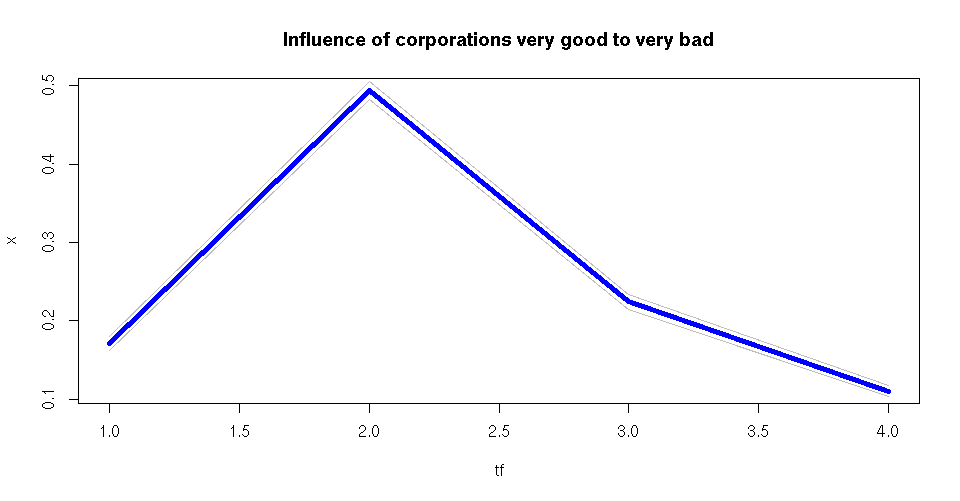
\includegraphics[scale=0.5]{corpop.png}

What this tells us is that even if we randomly sample ensuring that 25 nations are represented in each sample, there is a remarkable stability of the distribution and 66\% love corporations and 33\% hate them.

\section{Rethinking World Organisation Is Forced by Data}

Since we do want a peaceful world that addresses the legitimate natural demands of all people, my very strong result forces us to reconsider the issue of the sort of world we do want that can make all people in the world happy rather than only 66\% who love corporations.  The answer is not a severe anti-corporate revolution but something far more subtle.



\end{document}